\documentclass[a4paper,11pt]{article}
\usepackage{graphicx}
\usepackage{esvect}
\usepackage{subcaption}
\usepackage{listings}
\usepackage[top=0.75in, bottom=0.75in, left=0.6in, right=0.6in]{geometry}

\title{AE 625 - Particles Methods for Fluid Flow Simulation \\ SPH function and derivative approximation}
\author{Chillapalli Jyothi Durga Prasad - 140010042 }
\date{21 August 2017}

\usepackage{color}
 

\begin{document}
\maketitle


\tableofcontents
\listoffigures


\newpage
\section*{Consider Laney's problems and solve them using SPH.}
\indent The report is generated through the command \"\ sh a8-140010042.sh \"\\

\section{Solve $u_t+u_x=0$ with $u(x,0)=−sin(\pi x)$, periodic in [−1,1], find $u(x,40)$ using 40 points for discretization.\\}


\textbf{Results:}\\

\begin{figure}[ht]
    \centering
    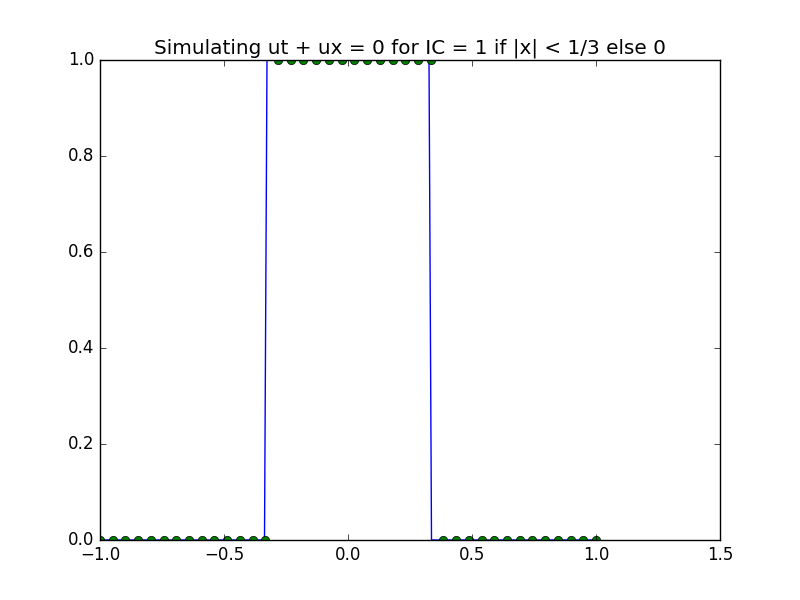
\includegraphics[width=.8\linewidth]{q2_40.png}
    \caption{Q1 40 points}
    \label{fig:ex1}    
\end{figure}

\begin{figure}[ht]
    \centering
    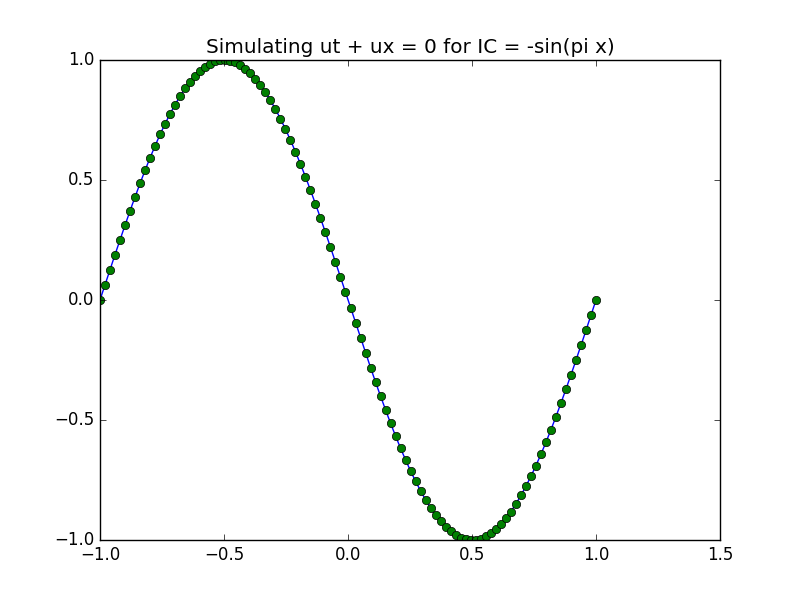
\includegraphics[width=.8\linewidth]{q1_100.png}
    \caption{Q1 100 points}
    \label{fig:ex2}    
\end{figure}
\newpage
\indent\\
\newpage
\section{Solve $u_t+u_x=0$ with $u(x,0)= 1 when  |x|<1/3 and 0 otherwise$, periodic in [−1,1], find $u(x,40)$ using 40 points for discretization.\\}

\textbf{Results:}\\

\begin{figure}[ht]
    \centering
    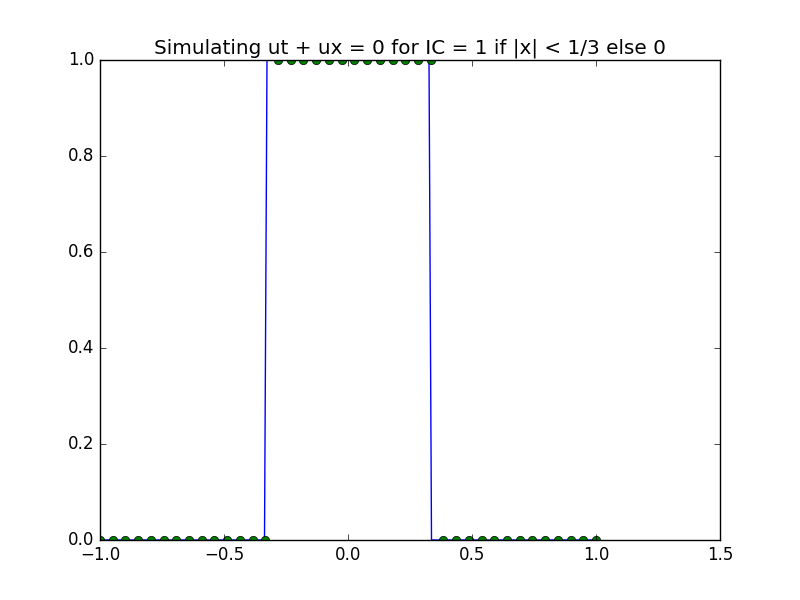
\includegraphics[width=.8\linewidth]{q2_40.png}
    \caption{Q2 40 points}
    \label{fig:ex3}    
\end{figure}

\begin{figure}[ht]
    \centering
    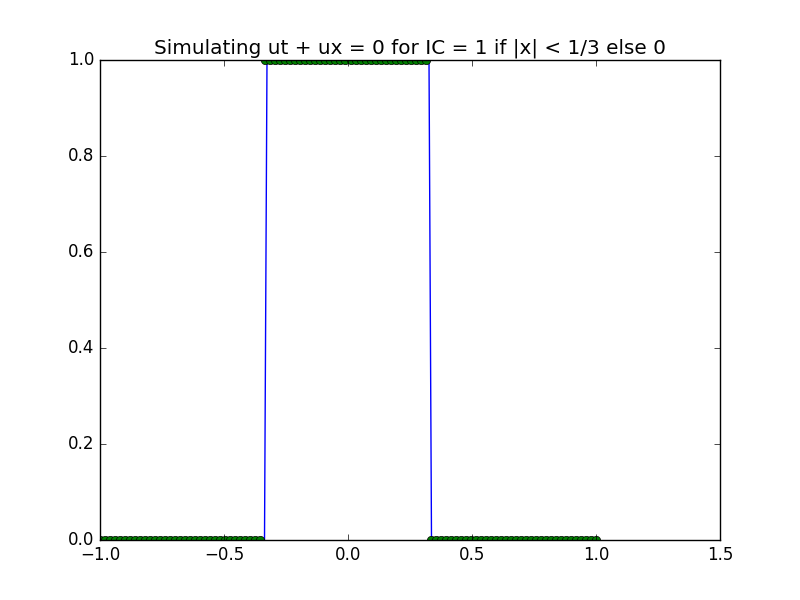
\includegraphics[width=.8\linewidth]{q2_100.png}
    \caption{Q2 100 points}
    \label{fig:ex4}    
\end{figure}
\newpage
\indent\\
\newpage
\indent\\

\section{Solve $u_t+u_x=0$ with $u(x,0)= 1 when  |x|<1/3 and 0 otherwise$, periodic in [−1,1], find $u(x,0.6)$ using 40 points for discretization.\\}

\textbf{Results:}\\

\indent \textbf{e = 0.5}
\begin{figure}[ht]
    \centering
    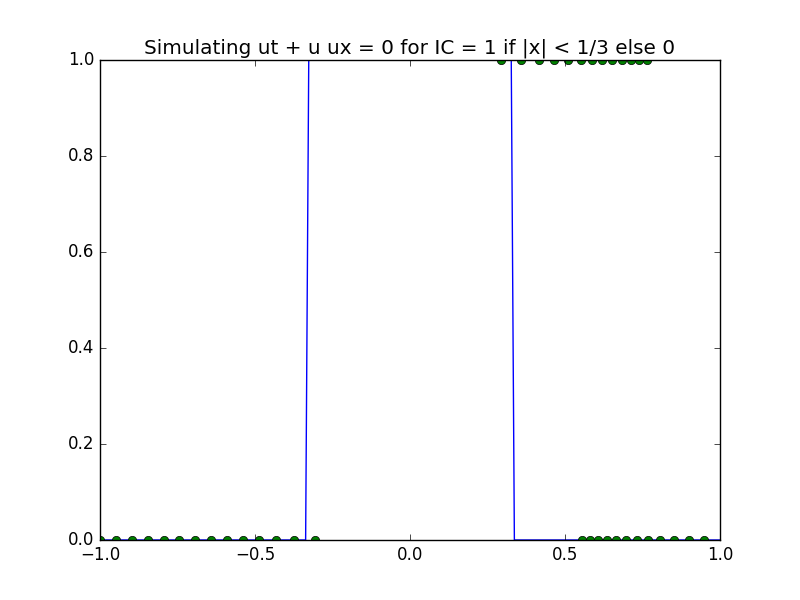
\includegraphics[width=.8\linewidth]{q3_40_05.png}
    \caption{Q3 40 e 0.5}
    \label{fig:ex5}    
\end{figure}

\begin{figure}[ht]
    \centering
    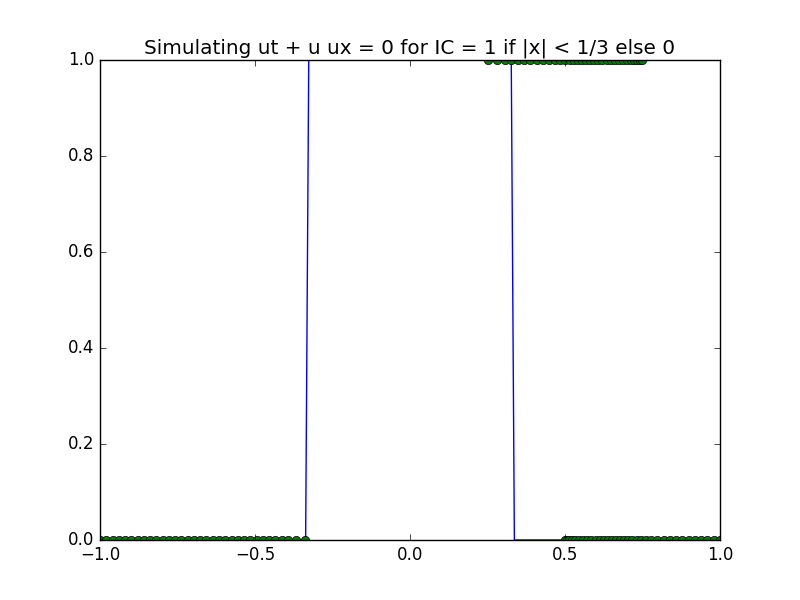
\includegraphics[width=.8\linewidth]{q3_100_05.png}
    \caption{Q3 100 e 0.5}
    \label{fig:ex6}    
\end{figure}
\newpage
\indent\\
\newpage
\indent \textbf{e = 1.0}
\begin{figure}[ht]
    \centering
    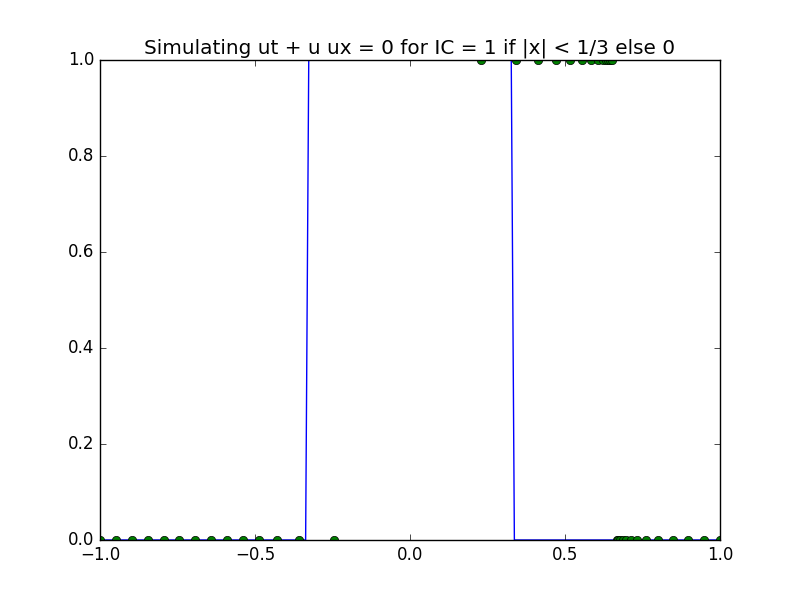
\includegraphics[width=.8\linewidth]{q3_40_1.png}
    \caption{Q3 40 e 1.0}
    \label{fig:ex7}    
\end{figure}

\begin{figure}[ht]
    \centering
    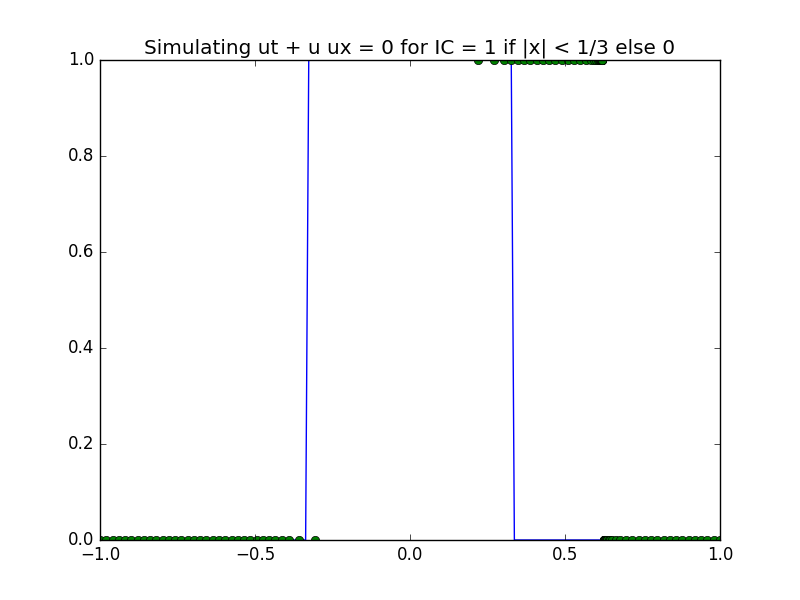
\includegraphics[width=.8\linewidth]{q3_100_1.png}
    \caption{Q3 100 e 1.0}
    \label{fig:ex8}    
\end{figure}

\newpage
\indent\\
\newpage
\section{Solve $u_t+u_x=0$ with $u(x,0)= 1 when  |x|<1/3 and -1 otherwise$, periodic in [−1,1], find $u(x,0.3)$ using 40 points for discretization.\\}

\textbf{Results:}\\

\indent \textbf{e = 0.5}
\begin{figure}[ht]
    \centering
    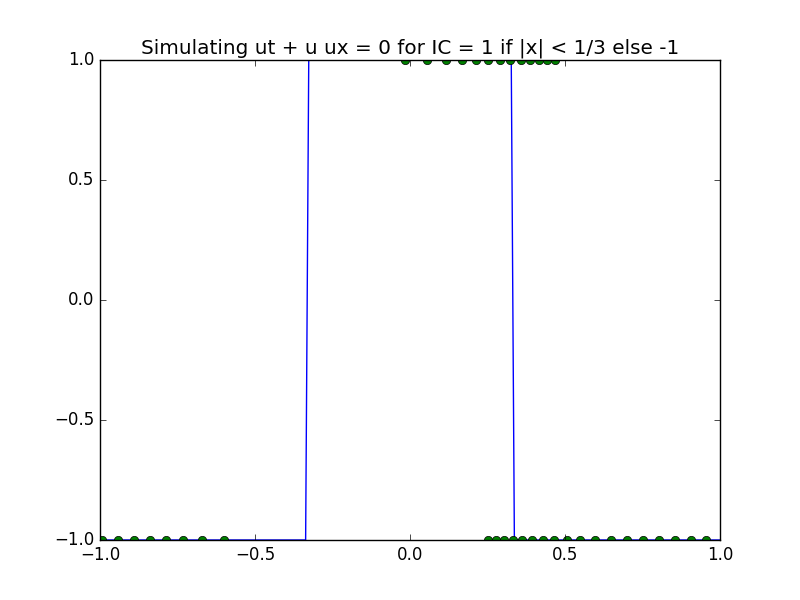
\includegraphics[width=.8\linewidth]{q4_40_05.png}
    \caption{Q4 40 e 0.5}
    \label{fig:ex9}    
\end{figure}

\begin{figure}[ht]
    \centering
    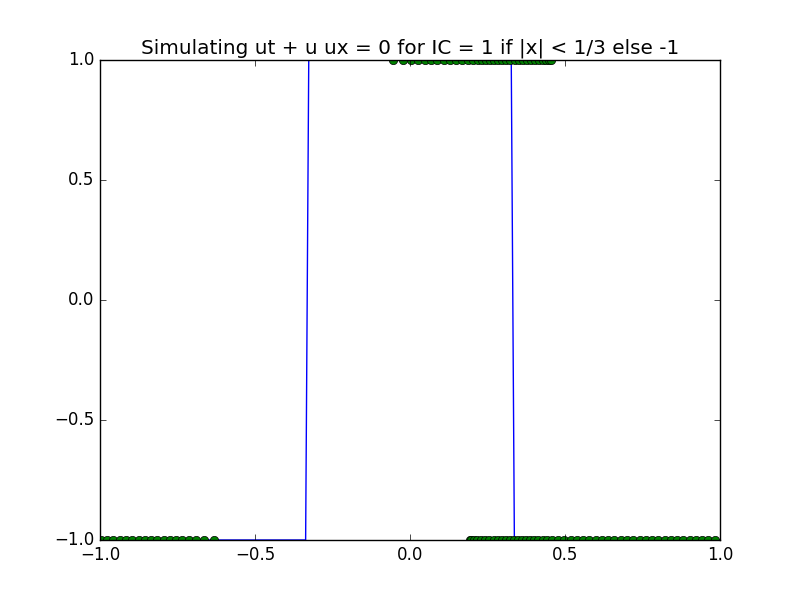
\includegraphics[width=.8\linewidth]{q4_100_05.png}
    \caption{Q4 100 e 0.5}
    \label{fig:ex10}    
\end{figure}
\newpage
\indent\\
\newpage
\indent \textbf{e = 1.0}
\begin{figure}[ht]
    \centering
    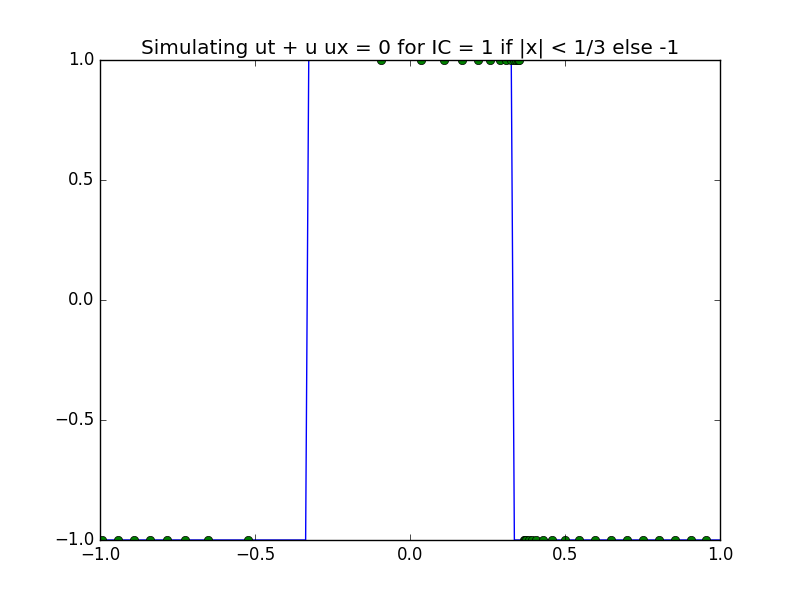
\includegraphics[width=.8\linewidth]{q4_40_1.png}
    \caption{Q4 40 e 1.0}
    \label{fig:ex11}    
\end{figure}

\begin{figure}[ht]
    \centering
    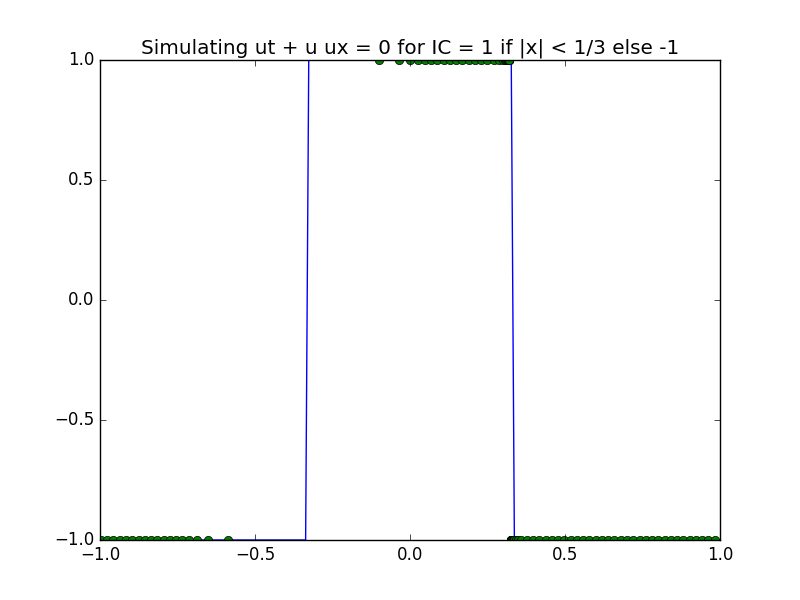
\includegraphics[width=.8\linewidth]{q4_100_1.png}
    \caption{Q4 100 e 1.0}
    \label{fig:ex12}    
\end{figure}

\newpage
\newpage
\textbf{Inference:}
\indent The XSPH velocity for e = 1.0 is nothing weighted average of velocity in the neighbourhood of x, So particles having same position will tend to move with same velocity as opposed to the case with e = 0.5 where particles retain a part of their original velocity\\



\end{document}
